%%%%%%%%%%%%%%%%%%%%%%%%%%%%%%%%%%%%%%%%%%%%%%%%%%%
%% Éléments flottants
%%%%%%%%%%%%%%%%%%%%%%%%%%%%%%%%%%%%%%%%%%%%%%%%%%%
%%%%%%%%%%%%%%%%%%
\section{Méthodologie de gestion du projet}
\subsection{Introduction}
\subsection{Étude préliminaire}
\subsubsection{Origine du génie logiciel}
\subsubsection{Comparaison des différentes méthodes de développement}
\subsubsubsection{Les approches traditionnelles}
\subsubsubsection{Les méthodes agiles}
\subsubsubsection{Synthèse}
\subsection{Conduite de projet}
\subsubsection{Modèle de livraison}
Aujourd'hui, Cegedim adopte une approche de livraison agile que tout projet est censé suivre. Le schéma ci-dessous montre les différentes phases de ce modèle (voir figure  ~\ref{fig:delivery}) :
\begin{figure}[H]
    \begin{center}
        \includegraphics[width=\linewidth]{images/sec3/deliveryprocess.pdf}
        \caption{Modèle de livraison}
        \label{fig:delivery}
    \end{center}
\end{figure}

\begin{figure}[H]
    \centering
        \includegraphics[width=0.68\linewidth]{images/sec3/organigrammedev.pdf}
        \caption{Organigramme DEV}
\end{figure}
{
\begin{center}
    \fboxsep=15pt\relax\fboxrule=4pt\relax%
    \vspace*{\fill}
    \specialbox{white}{actGreen}{31pt}{0.85\linewidth}{
        { \color{actGreen}
        \textbf{Responsable des développements}\\
        }
        {\footnotesize
        \begin{itemize}
            \item Accompagner le chef de projet dans la gestion des projets.
            \item Produire des indicateurs sur l’activité de développement.
            \item Suivi des risques et gestion des alertes.
            \item Travailler en collaboration avec les autres responsables de pôles.\\
        \end{itemize}}}
        \par\bigskip
        \specialbox{white}{actBlue}{31pt}{0.85\linewidth}{
            {
                \color{actBlue}\textbf{Chef de projet}\\
            }
            {\footnotesize\raggedright
            \begin{itemize}
                \item Valider les spécifications fonctionnelles.
                \item Assurer le suivi du processus de livraison et des indicateurs clés.
                \item Élaboration du plan de charge et planification des équipes.
                \item Garant des engagements (Qualité, Délai, Coût).\\
            \end{itemize}
        }}
        \par\bigskip
        \specialbox{white}{actPink}{31pt}{0.85\linewidth}{
            {
                \color{actPink}\textbf{Tech-Lead}\\
            }
            {\footnotesize\raggedright
            \begin{itemize}
                \item Responsable de la qualité technique (Audit, conception, etc.).
                \item Responsable des bonnes pratiques de développement.
                \item Encadrement et assistance technique.
                \item Participer aux développements.
                \item Assister le chef de projet pour les estimations de charge.\\
            \end{itemize}
        }}
        \par\bigskip
        \specialbox{white}{gray6}{31pt}{0.85\linewidth}{
            {
                \textbf{Ingénieur étude et développement}\\
            }
            {\footnotesize\raggedright
            \begin{itemize}
                \item Corriger les anomalies et développer de nouveaux modules.
                \item Respecter les bonnes pratiques de développement.
                \item Participer à la définition de la couverture de tests techniques.
                \item Rédiger des documents techniques.\\
            \end{itemize}
        }}
\end{center}    
}

\begin{figure}[H]
    \centering
        \includegraphics[width=0.52\linewidth]{images/sec3/organigrammeqa.pdf}
        \caption{Organigramme QA}
\end{figure}
{
\begin{center}
    \fboxsep=15pt\relax\fboxrule=4pt\relax%
    \specialbox{white}{actGreen}{31pt}{0.85\linewidth}{
        { \color{actGreen}
        \textbf{Responsable QA}\\
        }
        {\footnotesize
        \begin{itemize}
            \item Établir et piloter une stratégie de test.
            \item Accompagner le Team Lead dans la gestion des projets.
            \item Contribuer à l'amélioration des processus de test.
            \item Produire des indicateurs sur l’activité de testing.
            \item Suivi des risques et gestion des alertes.
            \item Travailler en collaboration avec les autres responsables de division.
        \end{itemize}}}
        \par\bigskip
        \specialbox{white}{actBlue}{31pt}{0.85\linewidth}{
            {
                \color{actBlue}\textbf{TL fonctionnel/technique}\\
            }
            {\footnotesize\raggedright
            \begin{itemize}
                \item Responsable du suivi du processus de livraison et des indicateurs clés.
                \item Élaboration du plan de charge et la planification des équipes.
                \item Accompagner et suivre les testeurs dans la mise en place des bonnes pratiques et des outils.
                \item Accompagner les ingénieurs QA dans l'élaboration des plans de test.
                \item Réaliser le bilan des activités.
                \item Accompagner l'intégration des nouveaux arrivants et veiller à la montée en compétence des équipes.
                \item Participer aux activités de test.\\
            \end{itemize}
        }}
        \par\bigskip
        \specialbox{white}{gray6}{31pt}{0.85\linewidth}{
            {
                \textbf{Ingénieur QA}\\
            }
            {\footnotesize\raggedright
            \begin{itemize}
                \item Formaliser les scénarios de test fonctionnels et automatisés.
                \item Valider et vérifier le développement de l’application.
                \item Respecter les bonnes pratiques de testing.
                \item Rédiger des documents fonctionnels.\\
            \end{itemize}
        }}
\end{center}    
}
\subsubsection{Déroulement du projet}
scrum
retrospective 
sprint
\subsubsection{Processus de développement}
specs fonctionnelles
codage
test unitaire
audit de code
documentation
\subsubsection{Gestion du workflow git}
Le workflow de travail pour les branches GIT choisi au niveau de Cegedim SRH est Gitflow. Git Flow est un modèle de dépôt git permettant d'améliorer les processus de développement et de mise en production d'un projet.\\
Voici un schéma présentant l'organisation du dépôt git ainsi que les différentes interactions qu'il peut y avoir entre chaque branche :
\subsection{Planification et suivi du projet}
La planification est parmi les phases d'avant-projet. Elle consiste non seulement à délimiter le périmètre temporel du projet, mais aussi à prévoir le déroulement des activités tout au long de la période allouée au stage.

\subsubsection{Diagramme de Gantt}
La figure suivante détaille la planification prévisionnelle du
projet (voir diagramme de Gantt figure 3.1).\\
\begin{figure}[H]
    \begin{center}
        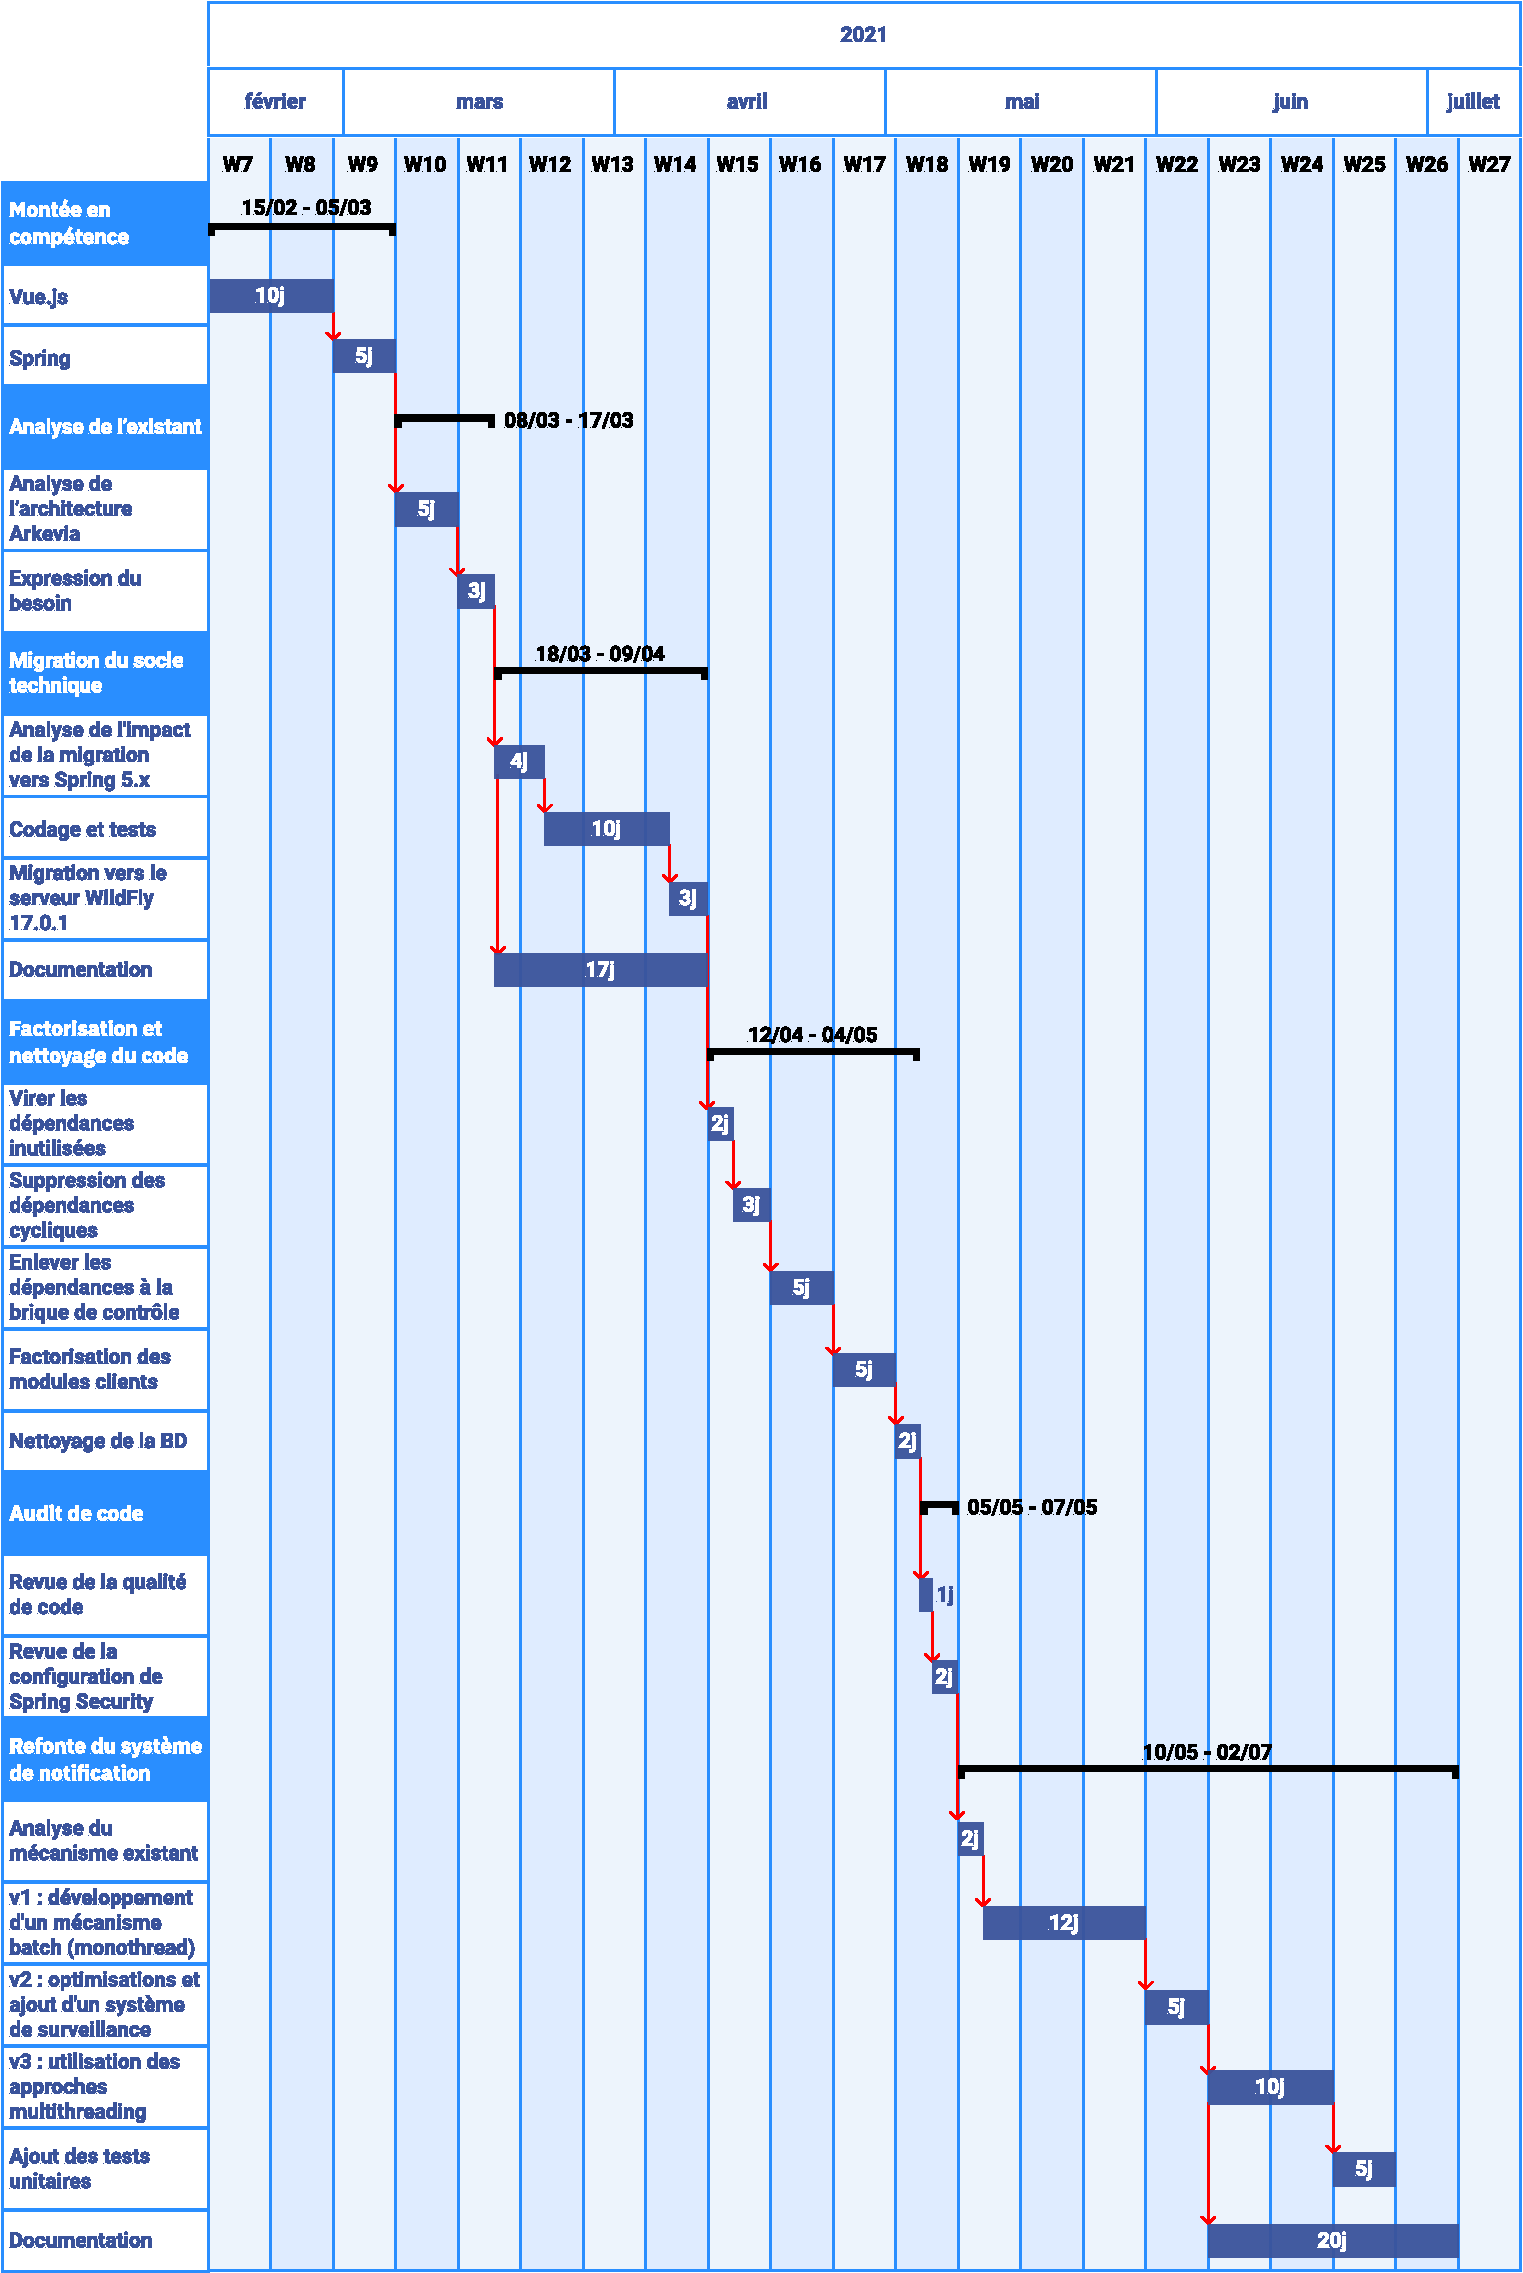
\includegraphics[width=\linewidth]{images/sec3/gantt.pdf}
        \caption{Diagramme de Gantt}
    \end{center}
\end{figure}
\subsection{Conclusion}
%%%%%%%%%%%%%%%%%%
